%--------------------
% Packages
% -------------------
\documentclass[11pt,a4paper]{article}
\usepackage[utf8x]{inputenc}
\usepackage[T1]{fontenc}
%\usepackage{gentium}
\usepackage{mathptmx} % Use Times Font
% \usepackage{wordcount}
\usepackage{listings}
\usepackage{amsmath}
\usepackage{minted}
\usepackage{pdflscape}
\usepackage[pdftex]{graphicx} % Required for including pictures
\usepackage[pdftex,linkcolor=black,pdfborder={0 0 0}]{hyperref} % Format links for pdf
\usepackage{calc} % To reset the counter in the document after title page
\usepackage[numbers]{natbib}
\usepackage{amssymb} % Required for \mathbb
\usepackage{amsmath} % Required for bmatrix environment
\frenchspacing % No double spacing between sentences
\linespread{1.2} % Set linespace
\usepackage[a4paper, lmargin=0.1666\paperwidth, rmargin=0.1666\paperwidth, tmargin=0.1111\paperheight, bmargin=0.1111\paperheight]{geometry} %margins
%\usepackage{parskip}

\usepackage[all]{nowidow} % Tries to remove widows
\usepackage[protrusion=true,expansion=true]{microtype} % Improves typography, load after fontpackage is selected
\newcommand{\apjs}{ApJS}
\newcommand{\apj}{ApJ}
\newcommand{\apjl}{ApJ}
\newcommand{\mnras}{MNRAS}
\newcommand{\aap}{A\&A}
\newcommand{\aj}{AJ}
\newcommand{\nat}{Nature}
\newcommand{\bain}{Bull.~Astron.~Inst.~Netherlands} 
\newcommand{\araa}{ARA\&A}
\newcommand{\icarus}{Icarus}
\setlength{\tabcolsep}{5pt} 
\renewcommand{\arraystretch}{0.8}

%-----------------------
% Set pdf information and add title, fill in the fields
%-----------------------
\hypersetup{ 	
pdfsubject = {Deep Learning Coursework},
pdftitle = {Deep Learning Coursework},
pdfauthor = {Laura Just Fung (lj441)}
}

\usepackage{hyperref}
\usepackage{cleveref}

%-----------------------
% Begin document
%-----------------------
\begin{document} 

\begin{center}
    \LARGE{\textbf{Deep Learning Coursework Assignment}}
    \\
    \Large{{Low-Rank Adaptation of Large Language Models for Time Series Forecasting}}
    \\
    \large{Laura Just Fung (lj441)}
    \\
    April 7, 2025
    \\
    Word count: 2196
\end{center}

\section{Introduction}
Time series forecasting is a challenging problem in machine learning when compared to other tasks such as image classification or natural language processing. This is because time series datasets are often comprised of incomplete data from different sources. Additionally, such problems often involve extrapolation from very small amounts of information \citep{gruver2024largelanguagemodelszeroshot}.

This report demonstrates that by encoding time series data as a string of digits, time series forecasting can be directly translated to next-token prediction in text. Thus, larga language models (LLMs) can be repurposed to this task fairly naturally, as shown by \citeauthor{gruver2024largelanguagemodelszeroshot}, who showed that LLMs are rather capable zero-shot time series forecasters. In this report, the Qwen2.5-0.5B-Instruct model \citep{yang2024qwen2technicalreport} along with Low-Rank Adaptation (LoRA) of the $q$ and $v$ projection matrices are used to explore this concept further and demonstrate performance of a LLM that has been fine-tuned towards this task.

\section{Compute constraints}
\label{sec:constraints}
A budget of $10^{17}$ floating point operations (FLOPS) was applied to this coursework, including all reported experiments as well as the final training run. The FLOPS accounting for primitives are defined in Table~\ref{tab:flops_primitives}. The extrapolated FLOPS for other operations are shown in Table~\ref{tab:flops_advanced}.
\renewcommand{\arraystretch}{1.2}
\begin{table}[h]
    \centering
    \begin{tabular}{c|c}
        Operations & FLOPS \\
        \hline
        Addition/Subtraction/Negation & 1 \\
        Multiplication/Division/Inverse & 1 \\
        ReLU/Absolute value & 1 \\
        Exponentiation/Logarithm & 10\\
        Sine/Cosine/Square root & 10 \\
        
    \end{tabular}
    \caption{Standardised FLOPS for common primitive operations as defined for the rest of this report.}
    \label{tab:flops_primitives}
\end{table}

\begin{table}
    \centering
    \begin{tabular}{c|c}
        Operation & FLOPS \\
        \hline
        $M_{m \times n} \times M_{n \times p}$ matrix multiplication & $mp(2n-1)$\\
        SiLU($M_{m \times n}$)& $13mn$ \\
        RMSNorm($M_{m \times n}$) & $m(5n + 10)$ \\
        Softmax($M_{m \times m}$) & $m(12m-1)$\\
        Embedding RoPE($M_{m \times n}$) & $mn$ \\ 
        Rank $r$ LoRA($M_{m \times m}$) & $2rm^2$
    \end{tabular}
    \caption{Extrapolated FLOPS for operations done whilst training and validating the LLM with LoRA.}
    \label{tab:flops_advanced}
\end{table}
While Qwen2.5-0.5B-Instruct uses SwiGLU activations as well as Grouped Query Attention, the FLOPS for SiLU activations as well as standard multi-headed attention have been used to simplify the calculations. For similar reasons, it has been assumed that the FLOPS of backpropagation are exactly twice that of the forward pass. Additionally, for all reported FLOPS, any operations performed outside of the model are not included. Finally, the cost of computing the rotary positional encodings have been ignored.

Using Tables~\ref{tab:flops_primitives} and \ref{tab:flops_advanced}, a Python script to calculate the FLOPS of the model's hyperparameters and input size was created. The script is located in \texttt{src/flops.py} and is used to calculate the FLOPS for the model's training and inference 

\section{Preprocessing}
\label{zero}
A text-based numeric encoding method adapted from the time series data preprocesing scheme described by \citeauthor{gruver2024largelanguagemodelszeroshot} was implemented for all data given to Qwen2.5-0.5B-Instruct. This preprocessing ensures that the numeric sequences are appropriately formatted for the best performance of Qwen2.5-0.5B-Instruct's tokenizer and forecasting.

First, as the numeric values in the dataset may vary, to standardise the numeric range of the data and control the token length, a simple scaling was applied, as shown in Eq.~\ref{eq:scale}

\begin{equation}
    x'_t = \frac{x_t}{\alpha},
    \label{eq:scale}
\end{equation}
where $\alpha$ is chosen based on the distribution of the dataset.

Additionally, the scaled numeric values were rounded to a fixed number of decimal places to ensure uniformity and consistent representation when tokenized.

The data used for this coursework involves multivariate Lotka-Volterra time series data. Thus, the following encoding is used, as shown in Eq.~\ref{eq:encode}:

\begin{equation}
    \begin{pmatrix}
        P_0 & Q_0 \\
        P_1 & Q_1 \\
        \vdots & \vdots \\
        P_t & Q_t 
        \end{pmatrix}  
        \rightarrow P_0,Q_0;P_{1},Q_{1};\ldots;P_{t},Q_{t},
    \label{eq:encode}
\end{equation}
where $P_t$ refers to the prey value at time $t$ and $Q_t$ refers to the predator value at time $t$. The comma is used to separate the predator and prey values, while the semicolon is used to separate the time steps.

The code for this preprocessing is shown in Listing~\ref{lst:preprocess},
\begin{listing}
\inputminted[firstline=64, lastline=83]{python}{../src/preprocessor.py}
\caption{Function to preprocess the time series data. The function takes in the prey and predator values, the scaling factor $\alpha$, and the number of decimal places to round to. It returns the encoded string representation of the time series data.}
\label{lst:preprocess}
\end{listing}
and this function can be found in the \texttt{preprocessor.py} file in the \texttt{src} directory.

As an example for the results for this preprocessing implementation with $\alpha = 5$ and 3 decimal places, the time series is encoded as shown in Table.~\ref{tab:example}, with trailing zeros dropped.

\begin{table}
    \centering
    \begin{tabular}{c|c}
        Stage & Value \\
        \hline
        Raw data & $\begin{pmatrix} 1.1335121  & 1.1031258 \\ 0.55542254  & 1.2579137 \end{pmatrix}$ \\
        Scaled data & $\begin{pmatrix} 2.267 & 2.206 \\ 1.111 & 2.516 \end{pmatrix}$ \\
        Encoded data & 2.267,2.206;1.111,2.516 \\
        Tokenized data & [17,13,17,21,22,11,17,13,17,15,21,26,16,13,16,16,16,11,17,13,20,16]
    \end{tabular}
    \caption{Example of the preprocessing steps for two steps in the time series data. The raw data is scaled, encoded, and then tokenized.}
    \label{tab:example}
\end{table}

A second example is shown in Table~\ref{tab:example2}.

\begin{table}
    \centering
    \begin{tabular}{c|c}
        Stage & Value \\
        \hline
        Raw data & $\begin{pmatrix} 0.8521567 & 0.9479834   \\ 0.6482769  & 0.94272685  \end{pmatrix}$ \\
        Scaled data & $\begin{pmatrix} 2.267 & 2.206 \\ 1.111 & 2.516 \end{pmatrix}$ \\
        Encoded data & 1.704,1.896;1.297,1.885 \\
        Tokenized data & [16,13,22,15,19,11,16,13,23,24,21,26,16,13,17,24,22,11,16,13,23,23,20]
    \end{tabular}
    \caption{Another example of the preprocessing steps for two steps in the time series data. The raw data is scaled, encoded, and then tokenized.}
    \label{tab:example2}
\end{table}
\clearpage
\section{Baseline}
\label{sec:baseline}
Using the preprocessing method described in Section~\ref{zero}, the untrained Qwen2.5-0.5B-Instruct model was evaluated on the tokenized Lotka-Volterra time series data. The model was given the first 80 points in the time-series data and asked to predict the next 20 points, as shown in Fig.~\ref{fig:baseline_pred}. The model was evaluated using mean absolute error (MAE), mean squared error (MSE), the R2 score, and running mean squared error (RMSE) for both the predator and prey time series data. The metrics for system id 870 are shown in Table~\ref{tab:baseline} and Fig.~\ref{fig:baseline_rmse}.

\begin{figure}[h]
    \centering
    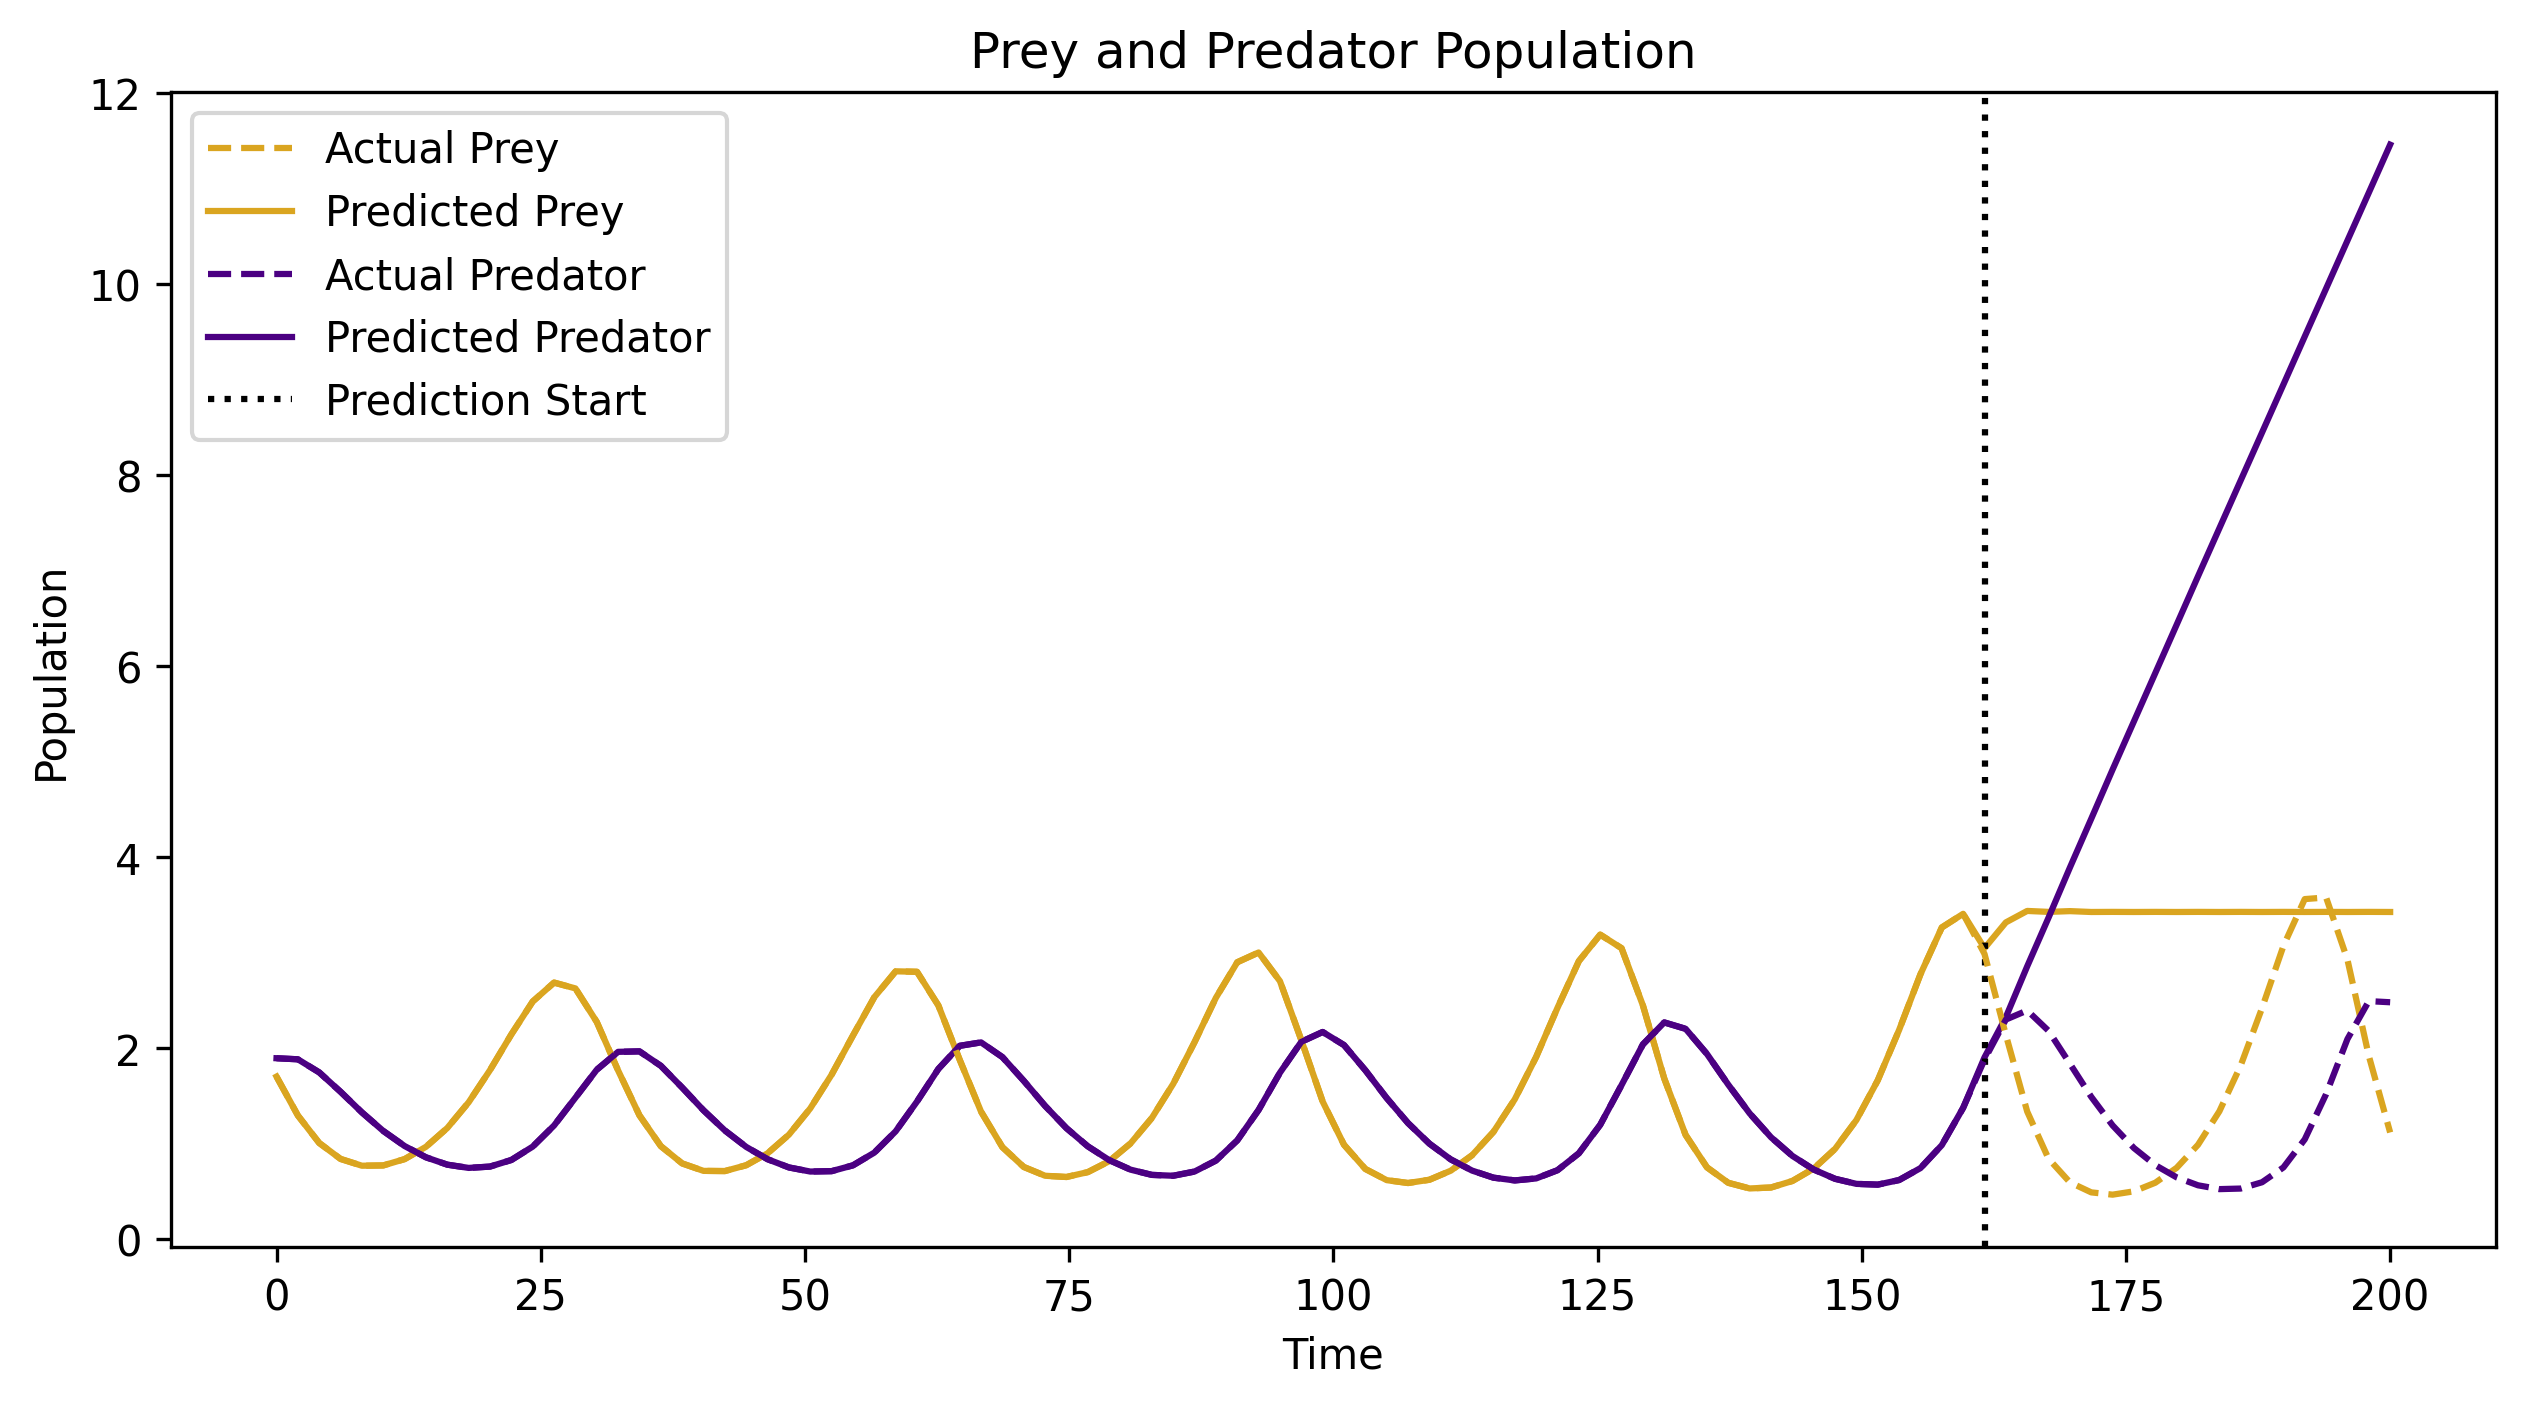
\includegraphics[width=\columnwidth, keepaspectratio]{../plots/predictions_example.png}
    \caption{Predictions of the untrained Qwen2.5-0.5B-Instruct model on system 870 of the Lotka-Volterra time series data. The model was given the first 80 points in the time-series data and asked to predict the next 20 points for both the predator (purple) and prey (gold) time series. The model's predictions are shown in the solid lines, while the true values are shown in the dashed lines.}
    \label{fig:baseline_pred}
\end{figure}

\begin{table}
    \centering
    \begin{tabular}{c|c|c|c|c}
        & \multicolumn{2}{c|}{Overall} & \multicolumn{2}{|c}{Out of distribution only}\\
        Metric & Prey & Predator & Prey & Predator \\
        \hline
        MAE & 0.5 & 0.814 & 2.249& 4.072\\
        MSE & 1.245 & 4.383 & 6.226& 21.917\\
        R2 score & 0.145 & -0.106 & -330.734& -3.919\\
    \end{tabular}
    \caption{Metrics for the untrained Qwen2.5-0.5B-Instruct model performance on system 870 of the Lotka-Volterra time series data. The model was given the first 80 points in the time-series data and asked to predict the next 20 points. The metrics are calculated for both the overall time series and the out-of-distribution data only.}
    \label{tab:baseline}
\end{table}

\begin{figure}
    \centering
    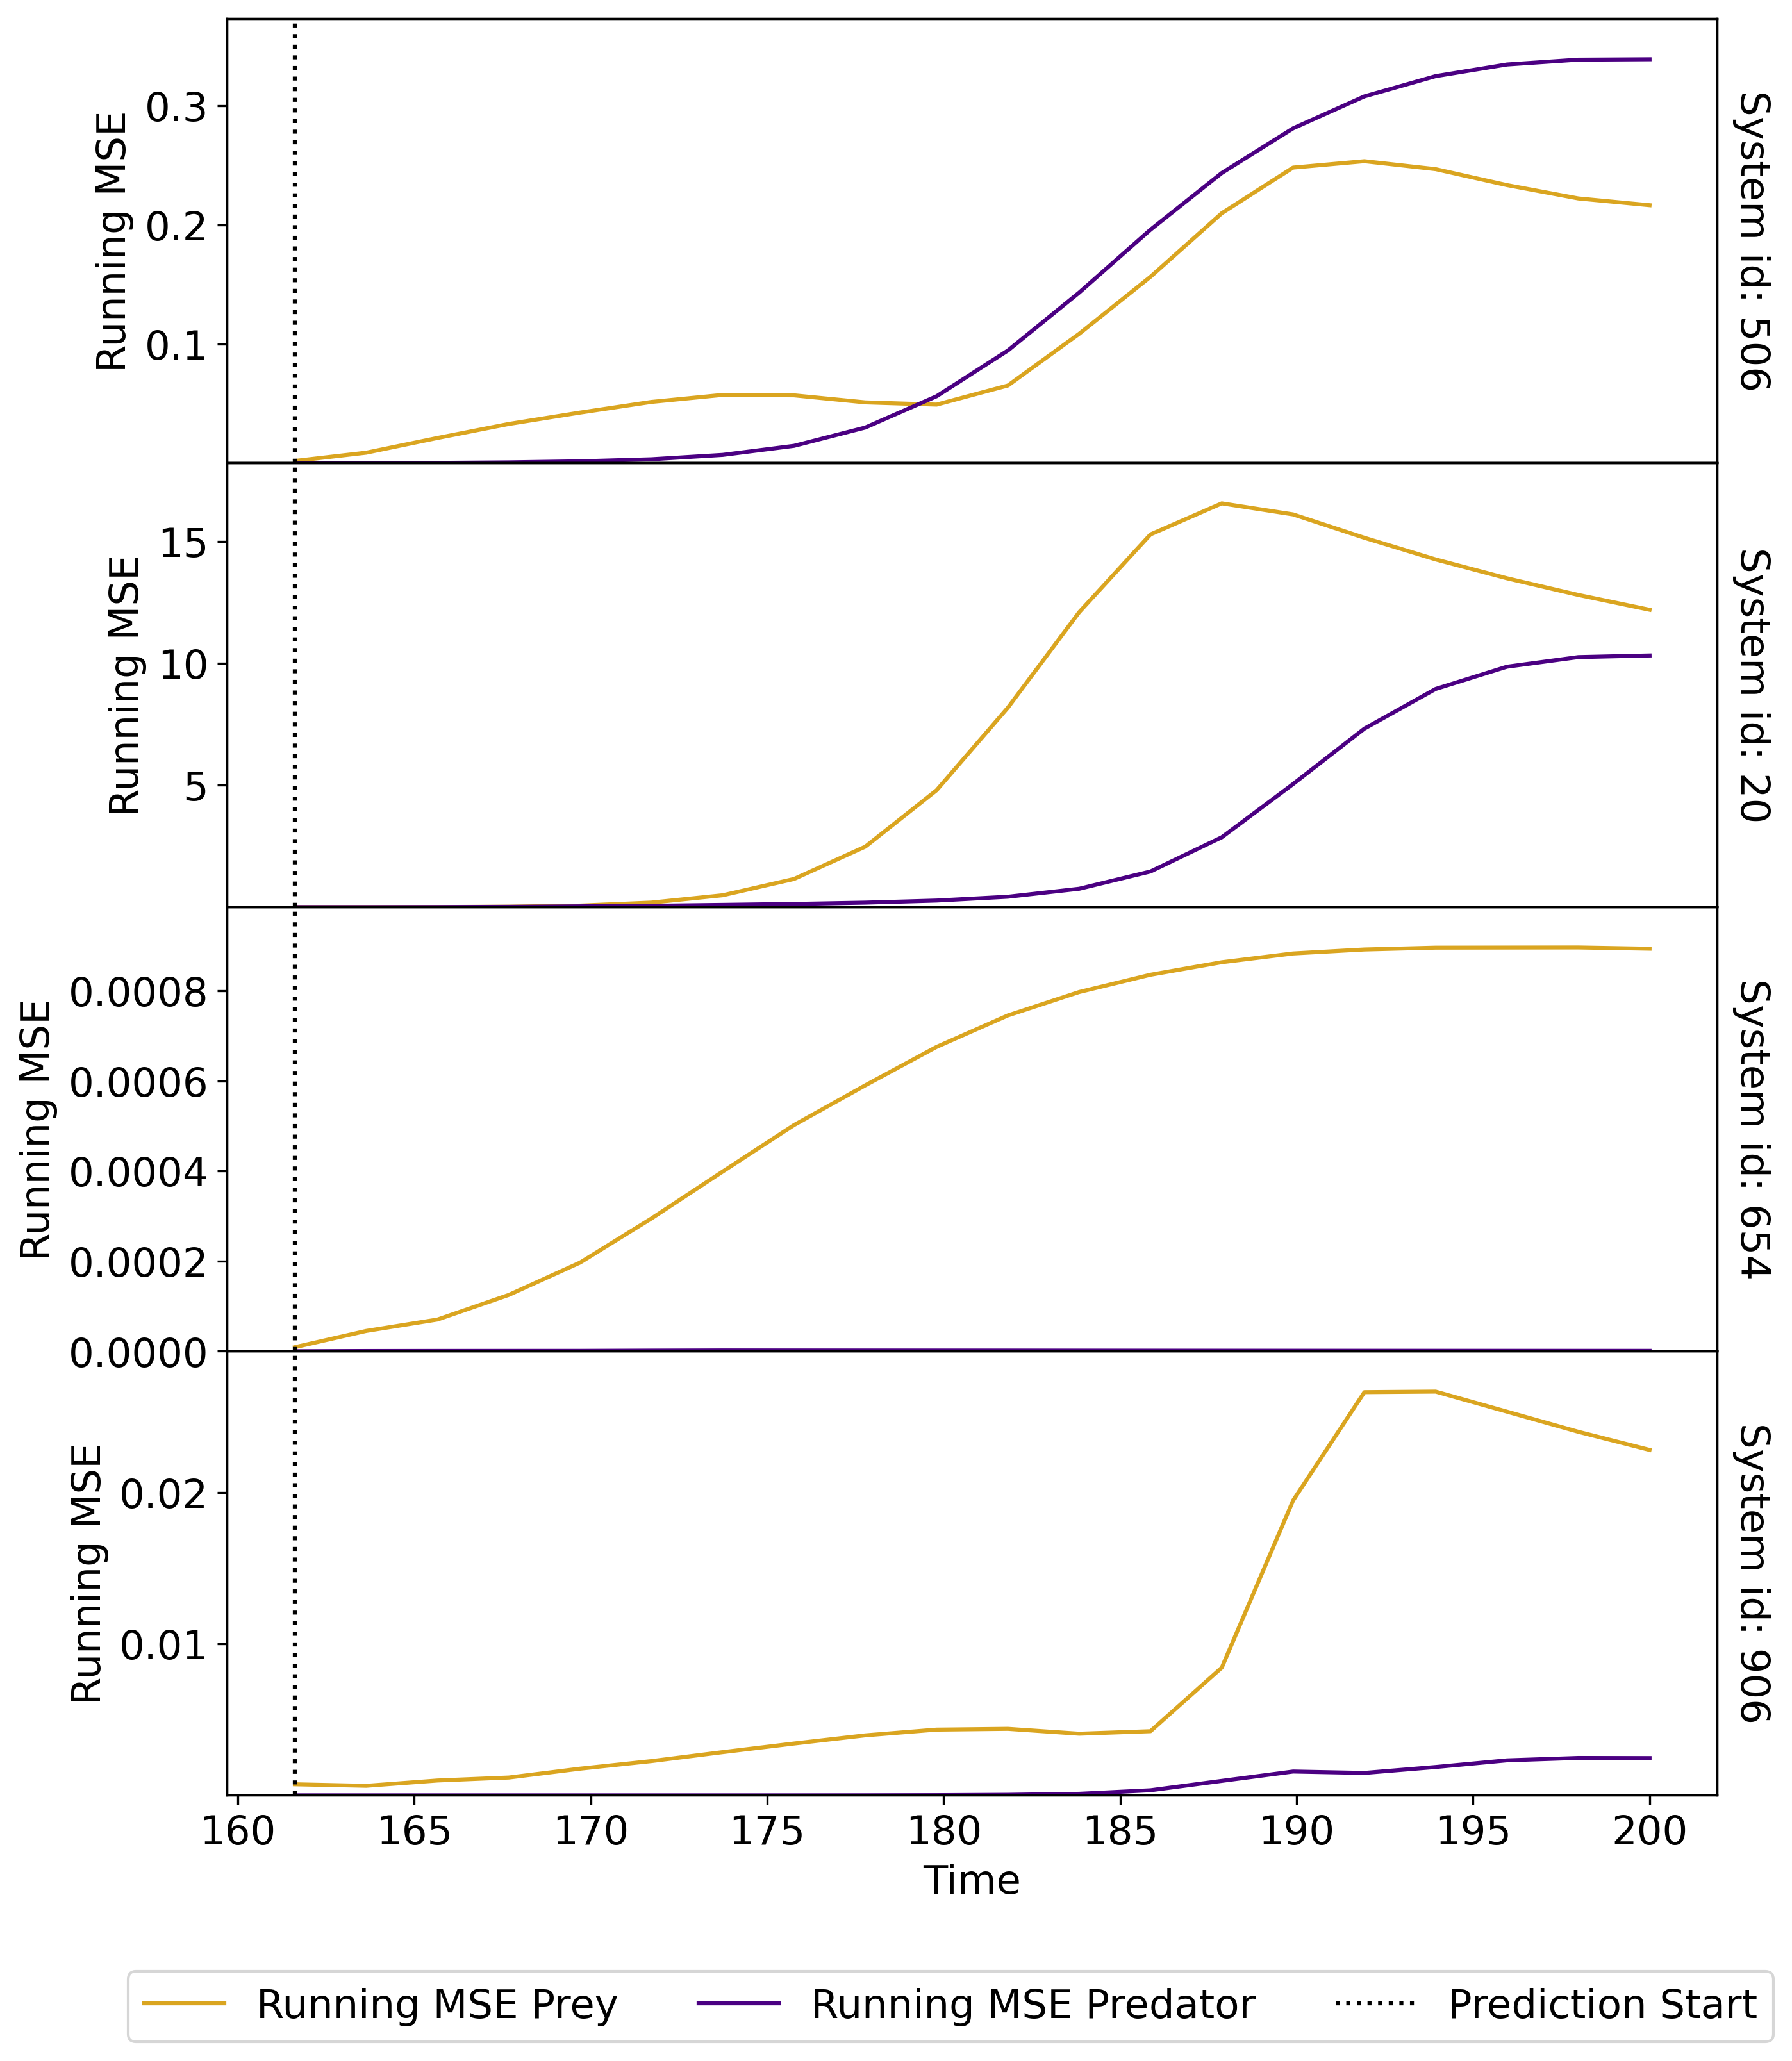
\includegraphics[width=\columnwidth, keepaspectratio]{../plots/running_mse_example.png}
    \caption{Running mean squared error (RMSE) for the untrained Qwen2.5-0.5B-Instruct model on system 870 of the Lotka-Volterra time series data. The model was given the first 80 points in the time-series data and asked to predict the next 20 points for both the predator (purple) and prey (gold) time series.}
    \label{fig:baseline_rmse}
\end{figure}

As can be seen in Fig.~\ref{fig:baseline_pred}, the untrained model is unable to predict the next 20 points in the time series data to any degree of accuracy. This is reflected in the metrics shown in Table~\ref{tab:baseline}, where the MAE and MSE for both predator and prey time series are very high, and the R2 score is either very low or negative. 
\clearpage
\bibliographystyle{vancouver-authoryear}
\bibliography{bibliography}
\appendix
\section{Use of auto-generation tools}
Auto-generation tools were used to help parse error messages throughout the project, and to help format this \LaTeX\ report.

Auto-generation tools were not used elsewhere, for code generation, writing, or otherwise.
\end{document}
